\chapter{Priority Queues \label{chap:prioqueue}}
Um den Begriff der  \emph{Priorit\"ats-Warteschlange} zu verstehen, betrachten wir zun\"achst
den Begriff der \emph{Warteschlange}.  Dort werden Daten hinten eingef\"ugt und vorne werden
Daten entnommen. Das f\"uhrt dazu, dass Daten in derselben Reihenfolge entnommen werden,
wie sie eingef\"ugt werden.  Anschaulich ist das so wie bei der Warteschlange vor einer
Kino-Kasse, wo die Leute in der Reihenfolge bedient werden, in der sie sich anstellen.
Bei einer Priorit\"ats-Warteschlange haben die Daten zus\"atzlich Priorit\"aten.  Es wird immer
das Datum entnommen, was die h\"ochste Priorit\"at hat.  Anschaulich ist das so wie im
Wartezimmer eines Zahnarztes. Wenn Sie schon eine Stunde gewartet haben und dann ein
Privat-Patient aufkreuzt, dann m\"ussen Sie halt noch eine Stunde warten, weil der
Privat-Patient eine h\"ohere Priorit\"at hat.

Priorit\"ats-Warteschlangen spielen in vielen Bereichen der Informatik  eine wichtige
Rolle.  Wir werden Priorit\"ats-Warteschlangen sp\"ater sowohl in dem Kapitel \"uber
Daten-Kompression als auch bei der Implementierung des Algorithmus zur Bestimmung
k\"urzester Wege in einem Graphen einsetzen.  Daneben werden Priorit\"ats-Warteschlangen unter anderem in
Simulations-Systemen und beim Scheduling von Prozessen in Betriebs-Systemen eingesetzt.


\section[Definition]{Definition des ADT \textsl{PrioQueue}}
Wir versuchen den Begriff der Priorit\"ats-Warteschlange jetzt formal durch Definition eines
abstrakten Daten-Typs zu fassen.
Wir geben hier eine eingeschr\"ankte Definition von Priorit\"ats-Warteschlangen, die nur die
Funktionen enth\"alt, die wir sp\"ater f\"ur den Algorithmus von Dijkstra ben\"otigen.
\begin{Definition}[Priorit\"ats-Warteschlange] \hspace*{\fill} \\
{\em
  Wir definieren den abstrakten Daten-Typ der \emph{Priorit\"ats-Warteschlange} wie folgt:
  \begin{enumerate}
  \item Als Namen w\"ahlen wir \textsl{PrioQueue}.
  \item Die Menge der Typ-Parameter ist \\[0.1cm]
        \hspace*{1.3cm} $\{ \textsl{Priority}, \textsl{Value} \}$.

        Dabei muss auf der Menge $\textsl{Priority}$ eine totale Quasi-Ordnung $<$ existieren,
        so dass wir die Priorit\"aten verschiedener Elemente vergleichen k\"onnen. 
  \item Die Menge der Funktions-Zeichen ist \\[0.1cm]
       \hspace*{1.3cm} 
       $\{ \textsl{prioQueue}, \textsl{insert}, \textsl{remove}, \textsl{top} \}$.
  \item Die Typ-Spezifikationen der Funktions-Zeichen sind gegeben durch:
        \begin{enumerate}
        \item $\textsl{prioQueue}: \textsl{PrioQueue}$

              Der Aufruf ``$\textsl{prioQueue}()$'' erzeugt eine leere
              Priorit\"ats-Warteschlange. 
        \item $\textsl{top}: \textsl{PrioQueue}  \rightarrow (\textsl{Priority} \times \textsl{Value}) \cup \{\Omega\}$

              Der Aufruf $Q.\textsl{top}()$ liefert ein Paar $\pair(p,v)$.  Dabei ist $v$ ein Element
              aus $Q$, das eine maximale Priorit\"at hat. $p$ ist die Priorit\"at des Elements $v$.
        \item $\textsl{insert}: \textsl{PrioQueue} \times \textsl{Priority} \times \textsl{Value} \rightarrow \textsl{PrioQueue}$

              Der Aufruf $Q.\textsl{insert}(p,v)$ f\"ugt das Element $v$ mit der Priorit\"at $p$ in
              die Priorit\"ats-Warteschlange $Q$ ein.  
        \item $\textsl{remove}: \textsl{PrioQueue} \rightarrow \textsl{PrioQueue}$

              Der Aufruf $Q.\textsl{remove}()$ entfernt aus der Priorit\"ats-Warteschlange
              $Q$ das Element, das durch den Ausdruck $Q.\texttt{top}()$ berechnet wird.
        \end{enumerate}
\item Bevor wir das Verhalten der einzelnen Methoden axiomatisch definieren, m\"ussen wir
      noch festlegen, was wir unter den \emph{Priorit\"aten} verstehen wollen, die den
      einzelnen Elementen aus $\textsl{Value}$ zugeordnet sind.  Wir nehmen an, dass die
      Priorit\"aten Elemente einer Menge $\textsl{Priority}$ sind und dass auf der Menge \textsl{Priority}
      eine totale Quasi-Ordnung $\leq$ existiert. Falls dann $p_1 < p_2$ ist, sagen wir, 
      dass $p_1$ eine h\"ohere Priorit\"at als $p_2$ hat.  Dies erscheint im ersten Moment vielleicht
      paradox. Es wird aber sp\"ater verst\"andlich, wenn wir den Algorithmus zur
      Berechnung k\"urzester Wege von Dijkstra diskutieren. Dort sind die Priorit\"aten
      Entfernungen im Graphen und die Priorit\"at eines Knotens ist um so h\"oher, je n\"aher
      der Knoten zu einem als \emph{Startknoten} ausgezeichneten Knoten ist. 

      Wir spezifizieren das Verhalten der Methoden nun dadurch, dass wir eine einfache
      \emph{Referenz-Implementierung} des ADT \textsl{PrioQueue} angeben und dann fordern,
      dass sich eine Implementierung des ADT \textsl{PrioQueue} genauso verh\"alt wie unsere
      Referenz-Implementierung.  Bei unserer Referenz-Implementierung stellen wir eine
      Priorit\"ats-Warteschlange durch eine Menge von Paaren von Priorit\"aten und Elementen 
      dar.   F\"ur solche Mengen definieren wir unserer Methoden wie folgt.
      \begin{enumerate}
      \item $\textsl{prioQueue}() = \{\}$,

             der Konstruktor erzeugt also eine leere
            Priorit\"ats-Warteschlange, die als leere Menge dargestellt wird. 
      \item $Q.\textsl{insert}(p, v) = Q \cup \{ \pair(p,v) \}$,
        
            Um ein Element $v$ mit einer Priorit\"at $p$ in die Priorit\"ats-Warteschlange 
            $Q$ einzuf\"ugen, reicht es aus, das Paar $\pair(p,v)$ zu der Menge $Q$ hinzuzuf\"ugen.
      \item Wenn $Q$ leer ist, dann ist $Q.\textsl{top}()$ undefiniert: \\[0.1cm]
            \hspace*{1.3cm} $Q = \{\} \;\rightarrow\; Q.\textsl{top}() = \Omega$.
     \item Wenn $Q$ nicht leer ist, wenn es also ein Paar $\pair(p_1, v_1)$ in $Q$
              gibt, dann liefert $Q.\textsl{top}()$ ein Paar $\pair(p_2,v)$ aus der Menge
              $Q$, so dass die Priorit\"at $p_2$ minimal wird.  Dann gilt also f\"ur
              alle $\pair(p_1,v_1) \in Q$, dass $p_2 \leq p_1$ ist.  Formal k\"onnen wir schreiben:
              \\[0.1cm]
              \hspace*{1.3cm} 
              $\pair(p_1,v_1) \in Q \;\wedge\; Q.\textsl{top}() = \pair(p_2,v_2)
              \;\rightarrow\; p_2 \leq p_1 \;\wedge\; \pair(p_2,v_2) \in Q$.
      \item Falls $Q$ leer ist, dann \"andert $\textsl{remove}()$ nichts daran: \\[0.1cm]
            \hspace*{1.3cm} $Q = \{\} \rightarrow Q.\textsl{remove}() = Q$.
      \item Sonst entfernt $Q.\textsl{remove}()$ das Paar, dass von $Q.\textsl{top}()$ berechnet wird: \\[0.1cm]
            \hspace*{1.3cm} 
            $Q \not= \{\} \rightarrow Q.\textsl{remove}() = Q \backslash \bigl\{ Q.\textsl{top}() \bigr\}$.
      \end{enumerate}
\end{enumerate}
}
\end{Definition}

Wir k\"onnen den abstrakten Daten-Typ \textsl{PrioQueue} dadurch implementieren,
dass wir eine Priorit\"ats-Warteschlange durch eine Liste realisieren, in der die Elemente
aufsteigend geordnet sind. Die einzelnen Operationen werden dann wie folgt implementiert:
\begin{enumerate}
\item $\textsl{prioQueue}()$ erzeugt eine leere Liste.
\item $Q.\textsl{insert}(d)$ kann durch die Prozedur \texttt{insert} implementiert werden,
      die wir beim ``\emph{Sortieren durch Einf\"ugen}'' entwickelt haben.
\item $Q.\textsl{top}()$ gibt das erste Element der Liste zur\"uck.
\item $Q.\textsl{remove}()$ entfernt das erste Element der Liste.
\end{enumerate}
Bei dieser Implementierung ist die Komplexit\"at der Operation $\textsl{insert}()$ 
linear in der
Anzahl $n$ der Elemente der Priorit\"ats-Warteschlange.  Alle anderen Operationen sind
konstant. Wir werden jetzt eine andere
Implementierung vorstellen, bei der die Komplexit\"at von $\textsl{insert}()$ 
 den Wert $\Oh\bigl(\log(n)\bigr)$ hat.  Dazu f\"uhren wir die Daten-Struktur eines
 \emph{Heaps} ein.

\section[Heaps]{Die Daten-Struktur \emph{Heap}}
Wir definieren die Menge \textsl{Heap}\footnote{
Der Begriff \textsl{Heap} wird in der Informatik f\"ur zwei v\"ollig unterschiedliche Dinge
verwendet:  Zum einen wird die in diesem Abschnitt beschriebene Daten-Struktur als
\textsl{Heap} bezeichnet, zum anderen wird der Teil des Speichers, in dem dynamisch
erzeugte Objekte abgelegt werden, ebenfalls als \textsl{Heap} bezeichnet.}
induktiv als Teilmenge der Menge $\Bin$ der
bin\"aren B\"aume. Dazu definieren wir zun\"achst f\"ur eine Priorit\"at $p_1\in \textsl{Priority}$ und
einen bin\"aren Baum $b \in \Bin$ die Relation $p_1 \leq b$ durch Induktion \"uber $b$.
Die Intention ist dabei, dass $p_1 \leq b$ genau dann gilt, wenn f\"ur jede Priorit\"at $p_2$,
die in $b$ auftritt,  $p_1 \leq p_2$ gilt. Die formale Definition ist wie folgt:
\begin{enumerate}
\item $p_1 \leq \textsl{Nil}$,

      denn in dem leeren Baum treten \"uberhaupt keine Priorit\"aten auf.
\item $p_1 \leq \textsl{Node}(p_2,v,l,r) \;\stackrel{\mbox{\scriptsize def}}{\longleftrightarrow}\; p_1 \leq p_2 \;\wedge\; p_1 \leq l \;\wedge\; p_1 \leq r$,
         
      denn $p_1$ ist genau dann kleiner-gleich als alle Priorit\"aten, die in dem Baum 
      $\textsl{Node}(p_2,v,l,r)$ auftreten, wenn $p_1 \leq p_2$ gilt und wenn zus\"atzlich
      $p_1$ kleiner-gleich als alle Priorit\"aten ist, die in $l$ oder $r$ auftreten.
\end{enumerate}
Als n\"achstes definieren wir eine Funktion \\[0.1cm]
\hspace*{1.3cm} $\textsl{count}: \Bin \rightarrow \mathbb{N}$, \\[0.1cm]
die f\"ur einen bin\"aren Baum die Anzahl der Knoten berechnet.  Die Definition erfolgt durch
Induktion:
\begin{enumerate}
\item $\textsl{Nil}.\textsl{count}() = 0$.
\item $\textsl{Node}(p,v,l,r).\textsl{count}() = 1 + l.\textsl{count}() + r.\textsl{count}()$.
\end{enumerate}
Mit diesen Vorbereitungen k\"onnen wir nun die Menge \textsl{Heap} induktiv definieren:
\begin{enumerate}
\item $\textsl{Nil} \in \textsl{Heap}$.
\item $\textsl{Node}(p,v,l,r) \in \textsl{Heap}$ g.d.w. folgendes gilt:
      \begin{enumerate}
      \item $p \leq l \;\wedge\; p \leq r$,

            Die Priorit\"at an der Wurzel ist also kleiner-gleich als alle anderen Priorit\"aten.
            Diese Bedingung bezeichnen wir auch als die \emph{Heap-Bedingung}.
      \item $\mid l.\textsl{count}() - r.\textsl{count}() \mid \;\leq\, 1$,

            Die Zahl der Elemente im linken Teilbaum ist also h\"ochstens 1 gr\"o{\ss}er oder
            kleiner als die Zahl der Elemente im rechten Teilbaum.
            Diese Bedingung bezeichen wir als die \emph{Balancierungs-Bedingung}.  Sie ist
            ganz \"ahnlich zu der Balancierungs-Bedingung bei AVL-B\"aumen, nur dass es dort
            die H\"ohe der B\"aume ist, die verglichen wird, w\"ahrend wir hier die Zahl der
            im Baum gespeicherten Elemente vergleichen.
      \item $l \in \textsl{Heap} \;\wedge\; r \in \textsl{Heap}$.
      \end{enumerate}
\end{enumerate}
Aus der \emph{Heap-Bedingung} folgt, dass ein nicht-leerer Heap die Eigenschaft hat, dass
das Element, welches an der Wurzel steht, immer die h\"ochste Priorit\"at hat.  Abbildung
\ref{fig:heap-list} auf Seite \pageref{fig:heap-list} zeigt einen einfachen Heap.
In den Knoten steht im oberen Teil die Priorit\"aten (in der Abbildung sind das nat\"urliche Zahlen) und
darunter stehen die Elemente (in der Abbildung sind dies Buchstaben).

\begin{figure}[!t]
  \centering
  \framebox{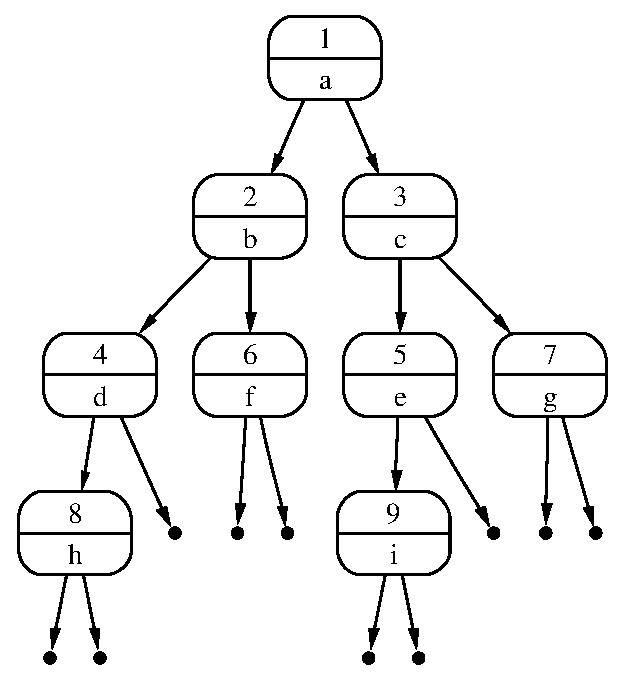
\epsfig{file=Abbildungen/heap-with-holes,scale=0.7}} 
  \caption{Ein Heap}
  \label{fig:heap-list}
\end{figure}


Da Heaps bin\"are
B\"aume sind, k\"onnen wir Sie ganz \"ahnlich wie geordnete bin\"are B\"aume  implementieren. 
Wir stellen zun\"achst Gleichungen auf, die die Implementierung der verschiedenen Methoden
beschreiben.  Wir beginnen mit der  Methode \textsl{top}.  Es gilt:
\begin{enumerate}
\item $\textsl{Nil}.\textsl{top}() = \Omega$.
\item $\textsl{Node}(p,v,l,r).\textsl{top}() = \pair(p,v)$,

      denn aufgrund der Heap-Bedingung wird das Element mit der h\"ochsten Priorit\"at 
      an der Wurzel gespeichert.
\end{enumerate}
Die Methoden \textsl{insert} m\"ussen wir nun so implementieren, dass
sowohl die Balancierungs-Bedingung als auch die Heap-Bedingung erhalten bleiben.
\begin{enumerate}
\item $\textsl{Nil}.\textsl{insert}(p,v) = \textsl{Node}(p,v,\textsl{Nil}, \textsl{Nil})$.
\item $p_{\mathrm{top}} \leq p \;\wedge\; l.\textsl{count}() \leq r.\textsl{count}() \;\rightarrow $   \\[0.1cm]
      \hspace*{1.3cm} 
      $\textsl{Node}(p_{\mathrm{top}},v_\mathrm{top},l,r).\textsl{insert}(p,v) =
                 \textsl{Node}\bigl(p_\mathrm{top},v_\mathrm{top},l.\textsl{insert}(p,v), r\bigr)$.

      Falls das einzuf\"ugende Paar eine geringere oder dieselbe Priorit\"at hat wie das
      Paar, welches sich an der Wurzel befindet, und falls zus\"atzlich die Zahl der Paare im linken Teilbaum
      kleiner-gleich der Zahl der Paare im rechten Teilbaum ist, dann f\"ugen wir das
      Paar im linken Teilbaum ein.
\item $p_{\mathrm{top}} \leq p \;\wedge\; l.\textsl{count}() > r.\textsl{count}() \;\rightarrow $   \\[0.1cm]
      \hspace*{1.3cm} 
      $\textsl{Node}(p_{\mathrm{top}},v_\mathrm{top},l,r).\textsl{insert}(p,v) =
                 \textsl{Node}\bigl(p_\mathrm{top},v_\mathrm{top},l,r.\textsl{insert}(p,v)\bigr)$.

      Falls das einzuf\"ugende Paar eine geringere oder dieselbe Priorit\"at hat als das
      Paar an der Wurzel und falls zus\"atzlich die Zahl der Paare im linken Teilbaum
      gr\"o{\ss}er als die Zahl der Paare im rechten Teilbaum ist, dann f\"ugen wir das
      Paar im rechten Teilbaum ein.
\item $p_{\mathrm{top}} > p \;\wedge\; l.\textsl{count}() \leq r.\textsl{count}() \;\rightarrow $ \\[0.1cm]
      \hspace*{1.3cm} 
      $\textsl{Node}(p_{\mathrm{top}},v_\mathrm{top},l,r).\textsl{insert}(p,v) =
                 \textsl{Node}\bigl(p,v,l.\textsl{insert}(p_\mathrm{top},v_\mathrm{top}), r\bigr)$.

      Falls das einzuf\"ugende Paar eine h\"ohere Priorit\"at hat als das Paar an
      der Wurzel, dann m\"ussen wir das neu einzuf\"ugende Paar an der Wurzel
      positionieren.  Das Paar, das dort vorher steht, f\"ugen wir in den linken
      Teilbaum ein, falls  die Zahl der Paare im linken Teilbaum
      kleiner-gleich der Zahl der Paare im rechten Teilbaum ist.
\item $p_{\mathrm{top}} > p \;\wedge\; l.\textsl{count}() > r.\textsl{count}() \;\rightarrow $ \\[0.1cm] 
      \hspace*{1.3cm} 
      $\textsl{Node}(p_{\mathrm{top}},v_\mathrm{top},l,r).\textsl{insert}(p,v) =
                 \textsl{Node}\bigl(p,v,l,r.\textsl{insert}(p_\mathrm{top},v_\mathrm{top})\bigr)$.

      Falls wir das einzuf\"ugende Paar an der Wurzel
      positionieren m\"ussen und die Zahl der Paare im linken Teilbaum
      gr\"o{\ss}er als die Zahl der Paare im rechten Teilbaum ist,
      dann m\"ussen wir das Paar, das vorher an der Wurzel stand, im rechten Teilbaum
      einf\"ugen.
\end{enumerate}
Als n\"achstes beschreiben wir die Implementierung der Methode \textsl{remove}.
\begin{enumerate}
\item $\textsl{Nil}.\textsl{remove}() = \textsl{Nil}$,

      denn aus dem leeren Heap ist nichts mehr zu entfernen.
\item $\textsl{Node}(p,v,\textsl{Nil},r).\textsl{remove}() = r$,
  
\item $\textsl{Node}(p,v,l,\textsl{Nil}).\textsl{remove}() = l$,

      denn wir entfernen immer das Paar mit der h\"ochsten Priorit\"at und das ist an der
      Wurzel.  Wenn einer der beiden Teilb\"aume leer ist, k\"onnen wir einfach den anderen
      zur\"uck geben.

      Jetzt betrachten wir die F\"alle, wo keiner der beiden Teilb\"aume leer ist.
      Dann muss entweder das Paar an der Wurzel des linken Teilbaums
      oder das Paar an der Wurzel des rechten Teilbaums an die Wurzel aufr\"ucken.
      Welches dieser beiden Paare wir nehmen, h\"angt davon ab, welches der Paare die h\"ohere
      Priorit\"at hat.
\item $p_1 \leq p_2 \;\wedge\; l = \textsl{Node}(p_1,v_1,l_1,r_1) \;\wedge\; r =
      \textsl{Node}(p_2,v_2,l_2,r_2) \;\rightarrow$ \\[0.1cm] 
      \hspace*{1.3cm} 
      $\textsl{Node}(p,v,l,r).\textsl{remove}() =      \textsl{Node}(p_1,v_1,l.\textsl{remove}(),r)$,

      denn wenn das Paar an der Wurzel des linken Teilbaums eine h\"ohere Priorit\"at hat
      als das Paar an der Wurzel des rechten Teilbaums, dann r\"uckt dieses Paar an
      die Wurzel auf und muss folglich aus dem linken Teilbaum gel\"oscht werden.
\item $p_1 > p_2 \;\wedge\; l = \textsl{Node}(p_1,v_1,l_1,r_1) \;\wedge\; r = \textsl{Node}(p_2,v_2,l_2,r_2) \rightarrow$ \\[0.1cm]
      \hspace*{1.3cm} 
      $\textsl{Node}(p,v,l,r).\textsl{remove}() = \textsl{Node}(p_2,v_2,l,r.\textsl{remove}())$,

      denn wenn das Paar an der Wurzel des rechten Teilbaums eine h\"ohere Priorit\"at hat
      als das Paar an der Wurzel des linken Teilbaums, dann r\"uckt dieses Paar an
      die Wurzel auf und muss folglich aus dem rechten Teilbaum gel\"oscht werden.  
\end{enumerate}
An dieser Stelle wird der aufmerksame Leser bemerken, dass die obige
Implementierung der Methode $\textsl{remove}()$ die Balancierungs-Bedingung verletzt.
Es ist nicht schwierig, die Implementierung so abzu\"andern, dass die
Balancierungs-Bedingung erhalten bleibt. Es zeigt sich jedoch, dass die
Balancierungs-Bedingung  nur beim Aufbau eines Heaps mittels \textsl{insert}() wichtig ist,
denn dort garantiert sie, dass die H\"ohe des Baums in logarithmischer Weise von der Zahl
seiner Knoten abh\"angt.  Beim L\"oschen wird die H\"ohe des Baums sowieso nur kleiner, also
brauchen wir uns da keine Sorgen machen.

\exercise
Change the equations for the method \texttt{remove} so that the resulting heap satisfies the
balancing condition.



\section[Implementation]{Implementing \textsl{Heaps} in \textsc{SetlX}}

\begin{figure}[bt]
\centering
\begin{Verbatim}[ frame         = lines, 
                  framesep      = 0.3cm, 
                  firstnumber   = 1,
                  labelposition = bottomline,
                  numbers       = left,
                  numbersep     = -0.2cm,
                  xleftmargin   = 0.0cm,
                  xrightmargin  = 0.0cm,
                ]
    class heap() {
        mPriority := om;
        mValue    := om;
        mLeft     := om;
        mRight    := om;
        mCount    := 0;
    
      static {
          top     := procedure()     { return [mPriority, mValue]; };
          insert  := procedure(p, v) { ... };
          remove  := procedure()     { ... };
          update  := procedure(t)    { ... };
          isEmpty := [] |-> mCount == 0;
      }
    }
\end{Verbatim}
\vspace*{-0.3cm}
\caption{Outline of the class \texttt{heap}.}
\label{fig:heap.stlx-outline}
\end{figure}

\noindent
Next, we present an implementation of heaps in \textsc{SetlX}. 
Figure \ref{fig:heap.stlx-outline} shows an outline of the class \texttt{heap}.  An object of class
heap represents a node in a heap data structure. In order to do this, it maintains the following
member variables:
\begin{enumerate}
\item \texttt{mPriority} is the priority of the value stored at this node,
\item \texttt{mValue}    stores the corresponding value,
\item \texttt{mLeft} and \texttt{mRight} represent the left and right subtree, respectively, while
\item \texttt{mCount}    gives the number of nodes in the subtree rooted at this node.
\end{enumerate}
The constructor initializes these member variables in a way that the resulting object represents an
empty heap.  Since a heap stores the value with the highest priority at the root, implementing the
method \texttt{top} is trivial: We just have to return the value stored at the root.
The implementation of \texttt{isEmpty} is easy, too: We just have to check whether the number of
values stored into this heap is zero.
\begin{figure}[!ht]
\centering
\begin{Verbatim}[ frame         = lines, 
                  framesep      = 0.3cm, 
                  firstnumber   = 1,
                  labelposition = bottomline,
                  numbers       = left,
                  numbersep     = -0.2cm,
                  xleftmargin   = 0.8cm,
                  xrightmargin  = 0.8cm,
                ]
    insert := procedure(priority, value) {
        if (isEmpty()) {
            this.mPriority := priority;
            this.mValue    := value;
            this.mLeft     := heap(this);
            this.mRight    := heap(this);
            this.mCount    := 1;
            return;
        }
        this.mCount += 1;
        if (priority < mPriority) {                         
            if (mLeft.mCount > mRight.mCount) {
                mRight.insert(mPriority, mValue);
            } else {
                mLeft.insert(mPriority, mValue);
            }
            this.mPriority := priority;
            this.mValue    := value;
        } else {
            if (mLeft.mCount > mRight.mCount) { 
                mRight.insert(priority, value);
            } else {
                mLeft.insert(priority, value);
            }
        }
    };
\end{Verbatim}
\vspace*{-0.3cm}
\caption{Implementation of the method \texttt{insert}.}
\label{fig:heap.stlx-insert}
\end{figure}

\noindent
Figure \ref{fig:heap.stlx-insert} show the implementation of the method \texttt{insert}.
Basically, there are two cases.
\begin{enumerate}
\item If the given heap is empty, then we store the value to be inserted at the current node.
      We have to make sure to set \texttt{mLeft} and \texttt{mRight} to empty heaps.  The reason is
      that, for every non-empty node, we want \texttt{mLeft} and \texttt{mRight} to store objects.
      Then, we can be sure that an expression like \texttt{mLeft.isEmpty()} is always well defined.
      If, however, we would allow \texttt{mLeft} to have the value \texttt{om}, then the evaluation
      of \texttt{mLeft.isEmpty()} would result in an error.
\item If the given heap is non-empty, we need another case distinction.
  \begin{enumerate}
  \item If the \texttt{priority} of the \texttt{value} to be inserted is higher\footnote{
        Remember that we have defined a priority $p_1$ to be \emph{higher} than a priority $p_2$
        iff $p_1 < p_2$.  I know that this sounds counter intuitive but unfortunately that is the
        way priorities are interpreted.  You will understand the reason for this convention later on
        when we discuss Dijkstra's \emph{shortest path algorithm}.}
        than
        \texttt{mPriority}, which is the priority of the value at the current node, then we have to 
        put \texttt{value} at the current node, overwriting \texttt{mValue}.  However, as we do not want
        to loose the value \texttt{mValue} that is currently stored at this node, we have to insert 
        \texttt{mValue} into either the left or the right subtree.  In order to keep the heap
        balanced we insert \texttt{mValue} into the smaller subtree and choose the left subtree if
        both subtrees have the same size.
  \item If the \texttt{value} to be inserted has a lower \texttt{priority} than \texttt{mPriority}, then we have
        to insert \texttt{value} into one of the subtrees.  Again, in order to maintain the balancing
        condition, \texttt{value} is stored into the smaller subtree.
  \end{enumerate}
\end{enumerate}

\begin{figure}[!ht]
\centering
\begin{Verbatim}[ frame         = lines, 
                  framesep      = 0.3cm, 
                  firstnumber   = 1,
                  labelposition = bottomline,
                  numbers       = left,
                  numbersep     = -0.2cm,
                  xleftmargin   = 0.8cm,
                  xrightmargin  = 0.8cm,
                ]
    remove := procedure() {
        this.mCount -= 1;
        if (mLeft.isEmpty()) { 
            update(mRight); 
            return;
        } 
        if (mRight.isEmpty()) { 
            update(mLeft ); 
            return;
        }
        if (mLeft.mPriority < mRight.mPriority) {
            this.mPriority := mLeft.mPriority;
            this.mValue    := mLeft.mValue;
            mLeft.remove();
        } else {
            this.mPriority := mRight.mPriority;
            this.mValue    := mRight.mValue;
            mRight.remove();
        }
    };
\end{Verbatim}
\vspace*{-0.3cm}
\caption{Implementation of the method \texttt{remove}.}
\label{fig:heap.stlx-remove}
\end{figure}

\noindent
Figure \ref{fig:heap.stlx-remove} shows the implementation of the method \texttt{remove}.  This
method removes the value with the highest priority from the heap.  Essentially, there are two
cases.
\begin{enumerate}
\item If the left subtree is empty, we replace the given heap with the right subtree. 
      Conversely, if the right subtree is empty, we replace the given heap with the  left subtree.
\item Otherwise, we have to check which of the two subtrees contains the value with the highest
      priority.  This value is then stored at the root of the given tree and, of course,
      it has to be removed from the subtree that had stored it previously.
\end{enumerate}

\begin{figure}[!ht]
\centering
\begin{Verbatim}[ frame         = lines, 
                  framesep      = 0.3cm, 
                  firstnumber   = 1,
                  labelposition = bottomline,
                  numbers       = left,
                  numbersep     = -0.2cm,
                  xleftmargin   = 0.8cm,
                  xrightmargin  = 0.8cm,
                ]
    update := procedure(t) {
        this.mPriority := t.mPriority;
        this.mValue    := t.mValue;
        this.mLeft     := t.mLeft;
        this.mRight    := t.mRight;
        this.mCount    := t.mCount;
    };      
\end{Verbatim}
\vspace*{-0.3cm}
\caption{Implementation of the method \texttt{update}.}
\label{fig:heap.stlx-update}
\end{figure}

\noindent 
Figure \ref{fig:heap.stlx-update} shows the implementation of the auxiliary method \texttt{update}.
Its implementation is straightforward: It copies the member variables stored at the node \texttt{t}
to the node \texttt{this}.  This method is needed since in \textsc{SetlX}, assignments of the form
\\[0.2cm]
\hspace*{1.3cm}
\texttt{this := mLeft;} \quad or \quad \texttt{this := mRight;}
\\[0.2cm]
are not permitted.
\pagebreak

\exercise
The implementation of the method \texttt{remove} given above violates the balancing condition.
Modify the implementation of \texttt{remove} so that the balancing condition remains valid.

\exercise
Instead of defining a class with member variables \texttt{mLeft} and \texttt{mRight}, a binary tree
can be stored as a list $l$.  In that case, for every index $i \in \{1, \cdots, \mathtt{\#}l \}$,
the expression $l[i]$ stores a node of the tree.  The crucial idea is that the left subtree of the
subtree stored at the index $i$ is stored at the index $2 \cdot i$, while the right subtree is
stored at the index $2 \cdot i + 1$.  Develop an implementation of heaps that is based on this idea.

%%% Local Variables: 
%%% mode: latex
%%% TeX-master: "algorithms"
%%% End: 
